\documentclass[11pt,a4paper]{article}

% --- Essential Packages ---
\usepackage[utf8]{inputenc}
\usepackage[a4paper, margin=0.85in, headheight=14pt, footskip=25pt]{geometry}
\usepackage{amsmath, amssymb, amsfonts}
\usepackage{graphicx}
\usepackage{booktabs}
\usepackage{tabularx}
\usepackage{xcolor}
\usepackage{listings}
\usepackage{fancyhdr}
\usepackage{lastpage}
\usepackage{hyperref}
\usepackage{titlesec}
\usepackage{tcolorbox}
\usepackage{enumitem}
\usepackage{float}
\usepackage{caption}

% --- Color Palette ---
\definecolor{primaryblue}{RGB}{30, 58, 138}    % Deep Navy Blue
\definecolor{accentblue}{RGB}{14, 116, 144}   % Teal / Slate Cyan
\definecolor{darktext}{RGB}{15, 23, 42}       % Dark Slate
\definecolor{lightbg}{RGB}{248, 250, 252}     % Slate 50
\definecolor{bordercolor}{RGB}{226, 232, 240} % Slate 200
\definecolor{alertred}{RGB}{185, 28, 28}      % Red 700
\definecolor{codebg}{RGB}{241, 245, 249}      % Slate 100
\definecolor{codecomment}{RGB}{100, 116, 139}% Slate 500
\definecolor{codestring}{RGB}{22, 101, 52}    % Green 800
\definecolor{codekeyword}{RGB}{124, 58, 237}  % Purple 600

% --- Hyperref Setup ---
\hypersetup{
    colorlinks=true,
    linkcolor=primaryblue,
    citecolor=accentblue,
    urlcolor=primaryblue,
    pdfauthor={Vishal Rawat, Jatin Nath, Rishi},
    pdftitle={Secure Chat Application - Cryptography and Network Security Project Report}
}

% --- Typography and Section Headings ---
\titleformat{\section}
  {\normalfont\Large\bfseries\color{primaryblue}}{\thesection}{1em}{}[{\titlerule[0.8pt]}]
\titleformat{\subsection}
  {\normalfont\large\bfseries\color{accentblue}}{\thesubsection}{1em}{}
\titleformat{\subsubsection}
  {\normalfont\normalsize\bfseries\color{darktext}}{\thesubsubsection}{1em}{}

% --- Header and Footer Styling ---
\pagestyle{fancy}
\fancyhf{}
\fancyhead[L]{\small\color{codecomment}\textbf{ICS412: Cryptography \& Network Security}}
\fancyhead[R]{\small\color{codecomment}\textbf{Secure Chat Lab Report}}
\fancyfoot[L]{\small\color{codecomment}Vishal Rawat (2023BCS0101) $\cdot$ Jatin Nath (2023BCD0014) $\cdot$ Rishi (2023BCD0023)}
\fancyfoot[R]{\small\color{codecomment}Page \thepage\ of \pageref{LastPage}}
\renewcommand{\headrulewidth}{0.4pt}
\renewcommand{\footrulewidth}{0.4pt}

% --- Code Listing Configuration ---
\lstset{
    language=Python,
    backgroundcolor=\color{codebg},
    basicstyle=\ttfamily\scriptsize\color{darktext},
    keywordstyle=\bfseries\color{codekeyword},
    commentstyle=\itshape\color{codecomment},
    stringstyle=\color{codestring},
    numbers=left,
    numberstyle=\tiny\color{codecomment},
    numbersep=7pt,
    frame=single,
    rulecolor=\color{bordercolor},
    breaklines=true,
    breakatwhitespace=true,
    showstringspaces=false,
    tabsize=4,
    captionpos=b,
    xleftmargin=12pt,
    xrightmargin=5pt
}

% --- Custom Alert Box ---
\newtcolorbox{securitybox}[1]{
    colback=lightbg,
    colframe=primaryblue,
    coltitle=white,
    fonttitle=\bfseries,
    title=#1,
    arc=3mm,
    boxrule=1pt,
    left=8pt,
    right=8pt,
    top=6pt,
    bottom=6pt
}

\newtcolorbox{warningbox}[1]{
    colback=lightbg,
    colframe=alertred,
    coltitle=white,
    fonttitle=\bfseries,
    title=#1,
    arc=3mm,
    boxrule=1pt,
    left=8pt,
    right=8pt,
    top=6pt,
    bottom=6pt
}

\begin{document}

% ==============================================================================
% TITLE & COVER PAGE
% ==============================================================================
\begin{titlepage}
    \pagenumbering{gobble}
    \centering
    \vspace*{0.5cm}
    
    {\huge \bfseries \color{primaryblue} Cryptography and Network Security (ICS412)\par}
    \vspace{0.4cm}
    {\Large \textsc{Course Project Report}\par}
    
    \vspace{1.2cm}
    \rule{\linewidth}{1.5pt}\par
    \vspace{0.4cm}
    {\huge \bfseries \color{darktext} Secure Chat Application using Diffie-Hellman Key Exchange, AES-256-CBC, and HMAC-SHA256\par}
    \vspace{0.3cm}
    {\large \bfseries \color{accentblue} With Real-Time Network Attack Simulation and Dynamic Adversarial Workbench\par}
    \vspace{0.4cm}
    \rule{\linewidth}{1.5pt}\par

    \vspace{1.8cm}

    {\Large \textbf{Submitted By:}\par}
    \vspace{0.4cm}
    
    \begin{table}[H]
        \centering
        \large
        \renewcommand{\arraystretch}{1.3}
        \begin{tabular}{lll}
            \textbf{Name} & \textbf{Roll Number} & \textbf{Program} \\
            \midrule
            \textbf{Vishal Rawat} & 2023BCS0101 & B.Tech Computer Science \& Engineering \\
            \textbf{Jatin Nath}   & 2023BCD0014 & B.Tech CSE (Data Science) \\
            \textbf{Rishi}        & 2023BCD0023 & B.Tech CSE (Data Science) \\
            \bottomrule
        \end{tabular}
    \end{table}

    \vfill

    {\large \textbf{Department of Computer Science and Engineering}\par}
    \vspace{0.2cm}
    {\large October 2026\par}
\end{titlepage}

% ==============================================================================
% ABSTRACT & TABLE OF CONTENTS
% ==============================================================================
\pagenumbering{roman}

\begin{abstract}
\noindent In contemporary computer networks, public communication channels are fundamentally untrusted and inherently susceptible to interception, manipulation, and spoofing. This project presents the design, mathematical formalization, and interactive implementation of an end-to-end secure communication system modeled after modern transport layer security protocols (such as TLS 1.3 and the Signal Protocol architecture). The system integrates four foundational pillars of modern applied cryptography:
\begin{enumerate}[leftmargin=1.5cm, label=\textbf{\arabic*.}]
    \item \textbf{Asymmetric Key Exchange:} Diffie-Hellman protocol based on RFC 3526 2048-bit MODP safe prime groups ($p, g$) to establish a shared master secret over an insecure channel without transmitting private exponents.
    \item \textbf{Key Derivation Function (KDF):} HMAC-based Extract-and-Expand Key Derivation Function (HKDF-SHA256, RFC 5869) to derive independent, cryptographically isolated 256-bit symmetric encryption keys ($K_{\text{AES}}$) and message authentication keys ($K_{\text{HMAC}}$).
    \item \textbf{Symmetric Payload Confidentiality:} Advanced Encryption Standard (AES-256) operating in Cipher Block Chaining (CBC) mode with cryptographically secure random Initialization Vectors (IV, 128-bit) per message and PKCS\#7 padding.
    \item \textbf{Message Integrity, Authentication, and Anti-Replay Defense:} Encrypt-then-MAC (EtM) paradigm utilizing HMAC-SHA256 computed over the 64-bit monotonically increasing sequence number, IV, and ciphertext payload ($\text{Seq} \parallel \text{IV} \parallel C$).
\end{enumerate}

To provide rigorous educational insight and empirical evaluation, the application embeds a real-time, tri-party visual environment containing Alice (sender), Bob (receiver), and Eve (network adversary). Through this platform, four critical adversarial scenarios are demonstrated: passive eavesdropping, ciphertext tampering (single-bit flipping), packet replay attacks, and unauthenticated Diffie-Hellman Man-in-the-Middle (MITM) interception. The system has been validated both as a standalone Python application leveraging Python \texttt{cryptography} primitives and as a zero-dependency web interface utilizing the W3C Web Cryptography API (\texttt{crypto.subtle}).
\end{abstract}

\vspace{0.5cm}
\tableofcontents
\newpage

\pagenumbering{arabic}

% ==============================================================================
% SECTION 1: INTRODUCTION
% ==============================================================================
\section{Introduction}

\subsection{Motivation and Problem Context}
The rapid proliferation of networked applications, distributed computing systems, and real-time messaging services has elevated information security from an operational feature to a critical architectural requirement. Open packet-switched networks (such as the Internet) inherently expose packets to inspection and unauthorized modification by intermediate entities, including untrusted routers, ISP taps, and active adversaries.

Achieving secure communication over an untrusted transmission medium necessitates fulfilling four fundamental security objectives defined by the CIA triad and extended cryptographic principles:
\begin{itemize}[leftmargin=1cm]
    \item \textbf{Confidentiality:} Preventing unauthorized disclosure of plaintext data to passive observers.
    \item \textbf{Integrity:} Ensuring that any modification, insertion, or deletion of transmitted data in transit is reliably detected by the recipient.
    \item \textbf{Authenticity \& Non-Repudiation:} Confirming that the received payload originates genuinely from the claimed peer entity.
    \item \textbf{Freshness \& Anti-Replay Defense:} Guaranteeing that previously intercepted valid packets cannot be maliciously retransmitted to induce state duplication or transaction replay.
\end{itemize}

\subsection{The Cryptographic Dilemma}
Symmetric ciphers such as AES-256 provide high-throughput, computationally lightweight encryption suitable for bulk data transfer. However, symmetric ciphers suffer from the fundamental \textbf{Key Distribution Problem}: two parties wishing to communicate must securely share a secret key beforehand. Transmitting the key across the open channel nullifies confidentiality.

Conversely, asymmetric (public-key) algorithms solve the key distribution dilemma through mathematically related key pairs but incur substantial computational overhead, rendering them impractical for streaming message encryption.

\subsection{Proposed Hybrid Architecture}
This project synthesizes asymmetric and symmetric paradigms into a \textbf{hybrid cryptographic architecture}:
\begin{enumerate}[leftmargin=1cm]
    \item \textbf{Diffie-Hellman (DH)} asymmetric key agreement establishes an ephemeral shared secret without disclosing the participants' private exponents.
    \item \textbf{HKDF-SHA256} stretches and separates the shared entropy into dedicated operational keys, eliminating cryptographic key-reuse vulnerabilities.
    \item \textbf{AES-256-CBC} secures arbitrary-length plaintexts using fresh initialization vectors.
    \item \textbf{HMAC-SHA256 (Encrypt-then-MAC)} binds message integrity and sequence counter tracking to the derived MAC key, thwarting chosen-ciphertext attacks, padding oracle vulnerabilities, and replay attacks.
    \item \textbf{Interactive Attack Workbench:} Eve's adversarial tap provides visibility into raw network packets, verifying that an adversary observes only pseudo-random bitstrings while interactively demonstrating failure modes when packets are corrupted or replayed.
\end{enumerate}

% ==============================================================================
% SECTION 2: SYSTEM ARCHITECTURE & THREAT MODEL
% ==============================================================================
\section{System Architecture \& Threat Model}

\subsection{Tri-Party System Architecture}
The system architecture consists of two legitimate communication endpoints (\textbf{Alice} and \textbf{Bob}) communicating across a shared, untrusted network tap controlled or observed by an adversary (\textbf{Eve}).

\begin{figure}[H]
    \centering
    \begin{tcolorbox}[colback=lightbg, colframe=bordercolor, width=0.92\linewidth, center]
    \centering\scriptsize\ttfamily
    \begin{tabular}{c c c}
    \textbf{ALICE (Sender)} & & \textbf{BOB (Receiver)} \\
    $\big\downarrow$ & & $\big\downarrow$ \\
    Priv: $a \in [2, p-2]$ & & Priv: $b \in [2, p-2]$ \\
    Pub: $A = g^a \pmod p$ & & Pub: $B = g^b \pmod p$ \\
    \midrule
    \multicolumn{3}{c}{\textbf{Insecure Public Network Channel (Dolev-Yao Wire)}} \\
    \multicolumn{3}{c}{$\Downarrow$} \\
    \multicolumn{3}{c}{\textbf{EVE (Adversary Tap: Sniff / Modify / Replay / MITM)}} \\
    \bottomrule
    \end{tabular}
    \end{tcolorbox}
    \caption{Conceptual tri-party network topology with active/passive adversary tap.}
    \label{fig:network_model}
\end{figure}

\subsection{Adversary Capabilities (Dolev-Yao Threat Model)}
We formalize Eve's capabilities under the canonical \textbf{Dolev-Yao threat model}:
\begin{itemize}[leftmargin=1cm]
    \item \textbf{Passive Eavesdropping:} Eve reads all raw bits transmitted across the wire ($A$, $B$, $\text{Seq}$, $\text{IV}$, $C$, and $\text{Tag}$).
    \item \textbf{Active Message Modification:} Eve can intercept and alter arbitrary bits of transmitted packets in transit before they reach the recipient.
    \item \textbf{Message Replay:} Eve can capture legitimate packets transmitted earlier and re-inject them into the network channel.
    \item \textbf{Man-in-the-Middle (MITM):} In the absence of digital signatures or public key infrastructure (PKI), Eve can intercept the public Diffie-Hellman values $A$ and $B$, replace them with her own parameters $Y_{E_1}, Y_{E_2}$, and establish distinct shared keys with Alice and Bob separately.
\end{itemize}

% ==============================================================================
% SECTION 3: CRYPTOGRAPHIC PROTOCOLS & MATHEMATICAL FORMULATIONS
% ==============================================================================
\section{Cryptographic Protocols \& Mathematical Formulations}

\subsection{Phase I: Diffie-Hellman Key Exchange (RFC 3526 Group 14)}
The Diffie-Hellman protocol operates over the multiplicative group of integers modulo a large safe prime $p$, where $p = 2q + 1$ (with $q$ prime) and $g$ is a generator of order $q$. In our implementation, we adopt RFC 3526 MODP Group 14 (2048-bit prime):
\begin{equation}
    \text{Group Parameters: } p \text{ (2048-bit safe prime)}, \quad g = 2
\end{equation}

\begin{enumerate}[leftmargin=1cm]
    \item \textbf{Private Exponent Selection:}
    \begin{align}
        \text{Alice chooses: } & a \xleftarrow{\mathcal{R}} [2, p-2] \\
        \text{Bob chooses: } & b \xleftarrow{\mathcal{R}} [2, p-2]
    \end{align}
    \item \textbf{Public Key Computation:}
    \begin{equation}
        A = g^a \pmod{p}, \qquad B = g^b \pmod{p}
    \end{equation}
    \item \textbf{Public Key Transmission:} Alice transmits $A$ to Bob; Bob transmits $B$ to Alice across the insecure channel.
    \item \textbf{Shared Secret Agreement:}
    \begin{align}
        \text{Alice computes: } & K_{\text{shared}} = B^a \pmod{p} = (g^b)^a \pmod{p} = g^{ab} \pmod{p} \\
        \text{Bob computes: } & K_{\text{shared}} = A^b \pmod{p} = (g^a)^b \pmod{p} = g^{ab} \pmod{p}
    \end{align}
\end{enumerate}

Due to the \textbf{Discrete Logarithm Problem (DLP)} and the \textbf{Computational Diffie-Hellman (CDH)} assumption, computing $g^{ab} \pmod{p}$ given $(p, g, A, B)$ is computationally intractable for 2048-bit modulus size within polynomial time.

\subsection{Phase II: Key Derivation Function (HKDF-SHA256, RFC 5869)}
The raw shared secret $K_{\text{shared}}$ from Diffie-Hellman is not uniformly distributed across its bit length. Using it directly as an AES key introduces potential key-schedule weaknesses. We employ HKDF-SHA256 (RFC 5869):
\begin{align}
    \text{PRK} &= \text{HMAC-SHA256}(\text{Salt}=\text{None}, K_{\text{shared}}) \\
    \text{OKM} &= \text{HKDF-Expand}(\text{PRK}, \text{info}=\text{"secure-chat-lab"}, L=64 \text{ bytes})
\end{align}

The 64-byte Output Keying Material (OKM) is partitioned into two distinct cryptographic keys:
\begin{align}
    K_{\text{AES}} &= \text{OKM}[0 \dots 31] \quad (\text{256-bit symmetric encryption key}) \\
    K_{\text{HMAC}} &= \text{OKM}[32 \dots 63] \quad (\text{256-bit message authentication key})
\end{align}

This strict key separation prevents cross-protocol cryptographic interactions and key reuse vulnerabilities.

\subsection{Phase III: AES-256-CBC Payload Confidentiality}
To encrypt an arbitrary plaintext message $M$:
\begin{enumerate}[leftmargin=1cm]
    \item \textbf{Sequence Number Tracking:} Increment the local 64-bit integer counter:
    \begin{equation}
        \text{Seq} \leftarrow \text{Seq} + 1
    \end{equation}
    \item \textbf{Initialization Vector (IV) Generation:} A fresh 128-bit random IV is generated using a cryptographically secure pseudo-random number generator (CSPRNG):
    \begin{equation}
        \text{IV} \xleftarrow{\mathcal{R}} \{0, 1\}^{128}
    \end{equation}
    \item \textbf{PKCS\#7 Padding:} Plaintext bytes $P$ are padded to a multiple of the 16-byte block size:
    \begin{equation}
        \text{PadLength} = 16 - (|P| \bmod 16)
    \end{equation}
    where each pad byte is filled with the integer value $\text{PadLength}$.
    \item \textbf{CBC Block Cipher Chaining:} For padded blocks $P_1, P_2, \dots, P_k$:
    \begin{align}
        C_0 &= \text{IV} \\
        C_i &= \text{AES-256}_{K_{\text{AES}}}(P_i \oplus C_{i-1}), \quad \forall i \in \{1, 2, \dots, k\} \\
        C &= C_1 \parallel C_2 \parallel \dots \parallel C_k
    \end{align}
\end{enumerate}

\subsection{Phase IV: Encrypt-then-MAC (EtM) Authentication}
Cryptographic consensus (Krawczyk, 2001; Bellare \& Namprempre, 2000) proves that \textbf{Encrypt-then-MAC} provides IND-CCA2 security and prevents padding oracle attacks:
\begin{equation}
    T = \text{HMAC-SHA256}_{K_{\text{HMAC}}}\left(\text{Seq}_{64} \parallel \text{IV}_{128} \parallel C\right)
\end{equation}
The serialized binary packet transmitted across the network is structured as:
\begin{equation}
    \text{Packet} = \underbrace{\text{Seq}}_{8\text{ bytes}} \;\parallel\; \underbrace{\text{IV}}_{16\text{ bytes}} \;\parallel\; \underbrace{C}_{N \times 16\text{ bytes}} \;\parallel\; \underbrace{T}_{32\text{ bytes}}
\end{equation}

\begin{figure}[H]
    \centering
    \begin{tcolorbox}[colback=codebg, colframe=bordercolor, width=0.95\linewidth, center]
    \centering\footnotesize\ttfamily
    \begin{tabular}{|c|c|c|c|}
    \hline
    \textbf{Seq (8 Bytes)} & \textbf{IV (16 Bytes)} & \textbf{Ciphertext ($N \times 16$ Bytes)} & \textbf{HMAC Tag (32 Bytes)} \\
    \hline
    Monotonic Counter & Random CSPRNG & AES-256-CBC Encrypted & HMAC-SHA256 (EtM) \\
    \hline
    \end{tabular}
    \end{tcolorbox}
    \caption{Wire packet layout ensuring confidentiality, authenticity, integrity, and freshness.}
    \label{fig:packet_structure}
\end{figure}

\subsection{Phase V: Receiver Decryption \& Anti-Replay Verification Pipeline}
Upon receipt of a network packet, the receiver executes a strict, defense-in-depth pipeline:

\begin{figure}[H]
    \centering
    \begin{tcolorbox}[colback=lightbg, colframe=primaryblue, width=0.92\linewidth, center]
    \centering\footnotesize\ttfamily
    Incoming Packet: [ Seq (8B) $\vert$ IV (16B) $\vert$ Ciphertext (NB) $\vert$ HMAC Tag (32B) ] \\
    $\Downarrow$ \\
    \textbf{1. HMAC-SHA256 Constant-Time Verification} \\
    $\text{HMAC}(K_{\text{HMAC}}, \text{Seq} \parallel \text{IV} \parallel C) \stackrel{?}{=} T$ \\
    $\swarrow$ \hspace{2cm} $\searrow$ \\
    \textbf{[PASS]} \hspace{2.5cm} \textbf{[FAIL]} $\rightarrow$ \textcolor{alertred}{\textbf{DROP PACKET! (Invalid Signature)}} \\
    $\downarrow$ \\
    \textbf{2. Anti-Replay Freshness Check} \\
    $\text{Seq} > \text{Recv\_Seq}$ ? \\
    $\swarrow$ \hspace{2cm} $\searrow$ \\
    \textbf{[PASS]} \hspace{2.5cm} \textbf{[FAIL]} $\rightarrow$ \textcolor{alertred}{\textbf{DROP PACKET! (Replay Detected)}} \\
    $\downarrow$ \\
    \textbf{3. AES-256-CBC Decryption \& PKCS\#7 Unpadding} \\
    $P = \text{Unpad}(\text{AES-Decrypt}(K_{\text{AES}}, C, \text{IV}))$ \\
    $\downarrow$ \\
    \textbf{4. Render Plaintext in Chat Window}
    \end{tcolorbox}
    \caption{Receiver verification pipeline. Integrity verification strictly precedes decryption.}
    \label{fig:pipeline_flow}
\end{figure}

\begin{securitybox}{Core Security Guarantee: Integrity Before Decryption}
Decryption is \textbf{never attempted} on untrusted ciphertext. Because the HMAC tag is verified in constant time first, any modified ciphertext or tampered byte is rejected immediately without parsing PKCS\#7 padding, mathematically neutralizing padding oracle attacks.
\end{securitybox}

% ==============================================================================
% SECTION 4: ATTACK SIMULATION MECHANISMS
% ==============================================================================
\section{Attack Simulation Mechanisms \& Defense Analysis}

The system incorporates interactive attack toggles enabling empirical validation of adversarial scenarios:

\begin{table}[H]
\centering
\small
\renewcommand{\arraystretch}{1.3}
\begin{tabularx}{\linewidth}{l >{\raggedright\arraybackslash}X >{\raggedright\arraybackslash}X}
\toprule
\textbf{Attack Scenario} & \textbf{Adversarial Mechanism} & \textbf{System Defense \& Detection} \\
\midrule
\textbf{Passive Eavesdropping} & Eve sniffs wire packets capturing $\text{Seq}, \text{IV}, C, T$. & Ciphertext exhibits maximum entropy. Without $K_{\text{AES}}$, decryption is computationally infeasible. \\
\addlinespace
\textbf{Active Ciphertext Tampering} & Eve flips a single bit in the ciphertext: $C[2] \leftarrow C[2] \oplus \text{0x01}$. & HMAC-SHA256 verification fails instantly. Packet dropped with explicit visual alert; decryption is aborted. \\
\addlinespace
\textbf{Packet Replay Attack} & Eve re-transmits a previously captured valid packet. & Sequence check fails ($\text{Seq} \le \text{Recv\_Seq}$). Packet dropped as duplicate/replay. \\
\addlinespace
\textbf{Man-in-the-Middle (MITM)} & Eve intercepts public parameters $A, B$ and substitutes $Y_{E_1}, Y_{E_2}$. & Demonstrates the vulnerability of unauthenticated DH. Highlights the requirement for X.509 certificates and PKI signatures. \\
\bottomrule
\end{tabularx}
\caption{Comprehensive breakdown of simulated attacks and corresponding defensive primitives.}
\label{tab:attack_matrix}
\end{table}

% ==============================================================================
% SECTION 5: EXPERIMENTAL RESULTS & SCREENSHOT EVALUATION
% ==============================================================================
\section{Experimental Results \& Screenshot Evaluation}

The application was empirically tested through both the Python Tkinter interface and the Web Cryptography interface. Below are test captures documenting each operational phase.

\subsection{Figure 1: Initial Application State (Channel Not Secured)}
\begin{figure}[H]
    \centering
    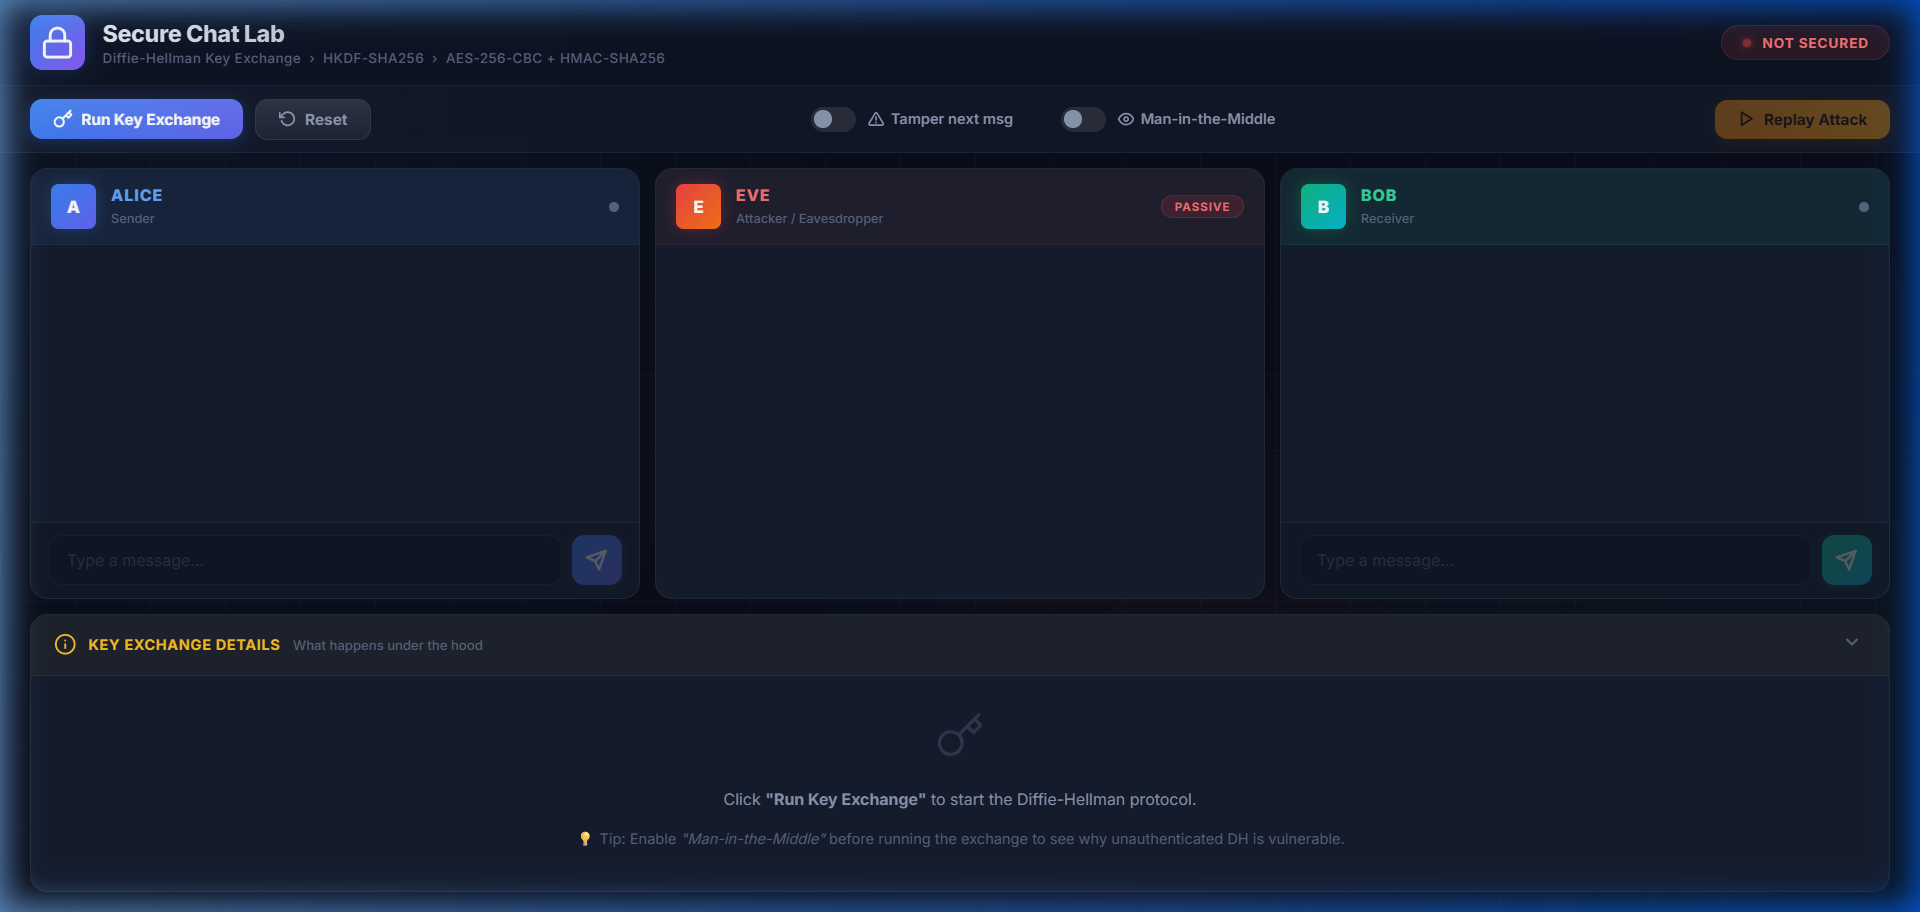
\includegraphics[width=0.88\linewidth]{screenshots/fig1_initial_state.png}
    \caption{Application interface at startup prior to cryptographic handshake.}
    \label{fig:exp_initial}
\end{figure}
\noindent \textbf{Analysis:} The interface displays Alice (blue, left), Bob (green, right), and Eve (red, center). Chat inputs remain locked until secure parameters are established. The status badge indicates \texttt{NOT SECURED}.

\newpage
\subsection{Figure 2: Step-by-Step Diffie-Hellman Key Exchange \& HKDF Derivation}
\begin{figure}[H]
    \centering
    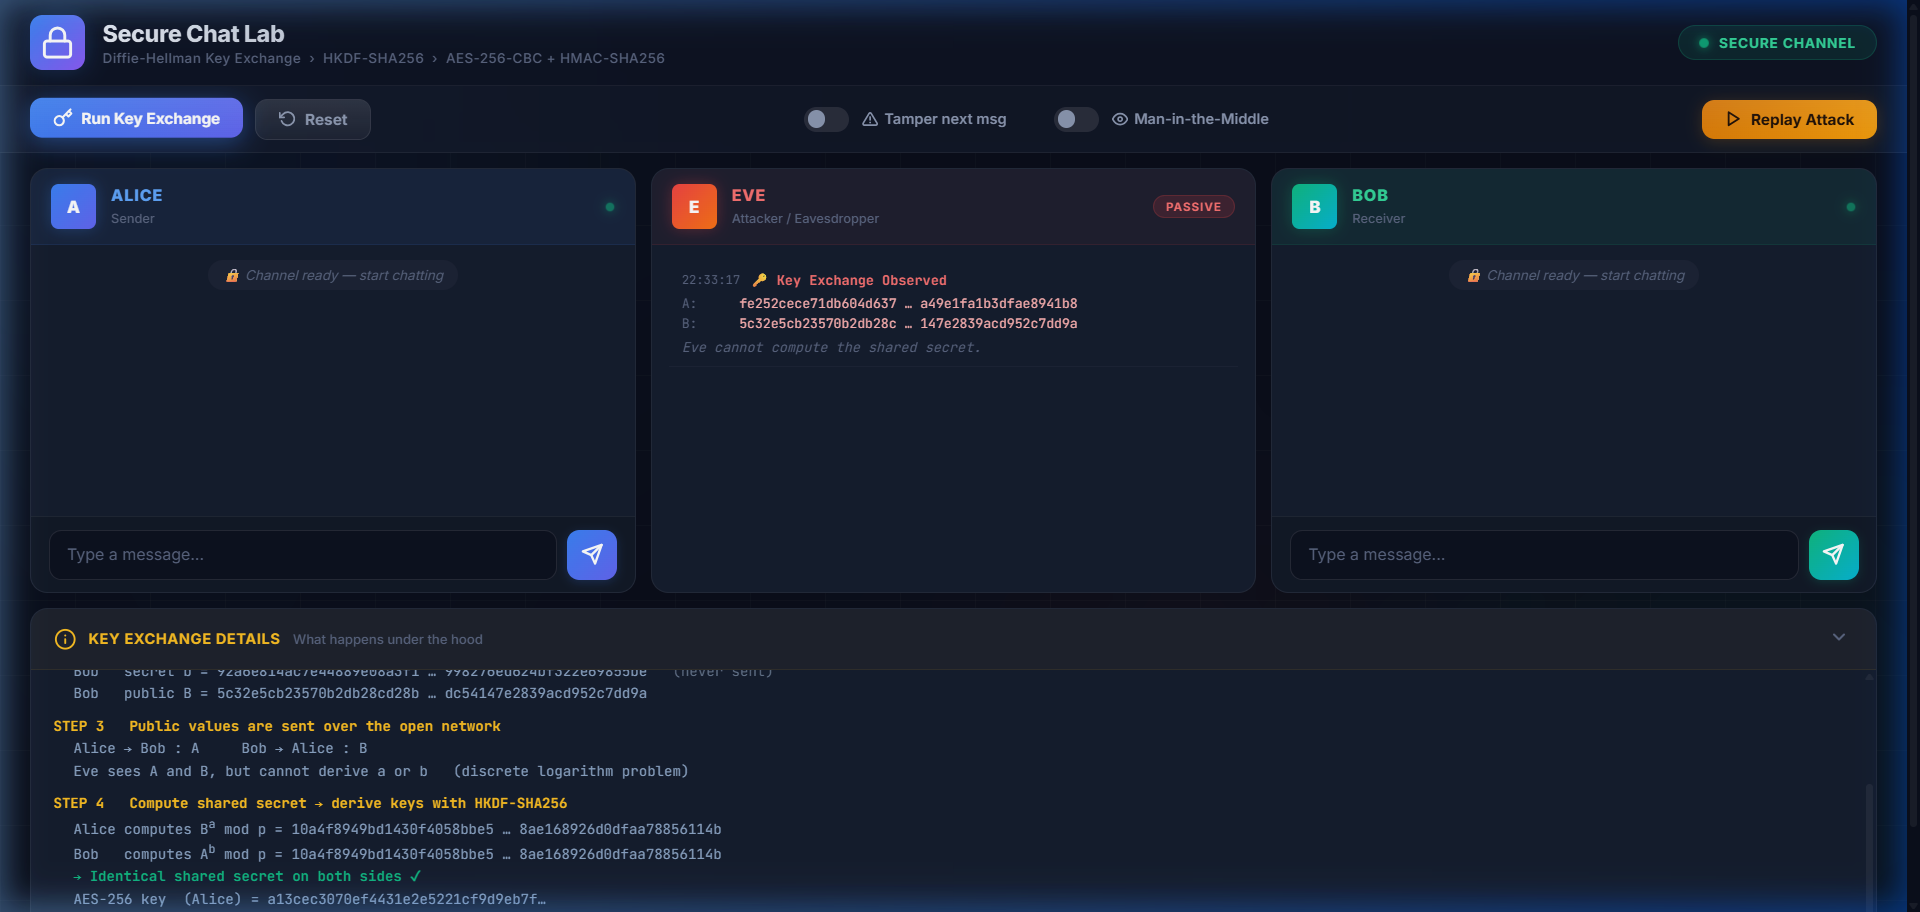
\includegraphics[width=0.88\linewidth]{screenshots/fig2_key_exchange.png}
    \caption{Execution of RFC 3526 DH Key Exchange and HKDF-SHA256 key expansion.}
    \label{fig:exp_kx}
\end{figure}
\noindent \textbf{Analysis:} The lower telemetry log details the 2048-bit prime $p$, generator $g=2$, private exponents $a$ and $b$, computed public values $A$ and $B$, shared secret $g^{ab} \pmod{p}$, and derived 256-bit AES and HMAC keys. The channel transitions to \texttt{SECURE CHANNEL}.

\subsection{Figure 3: Secure End-to-End Chat \& Eavesdropper View}
\begin{figure}[H]
    \centering
    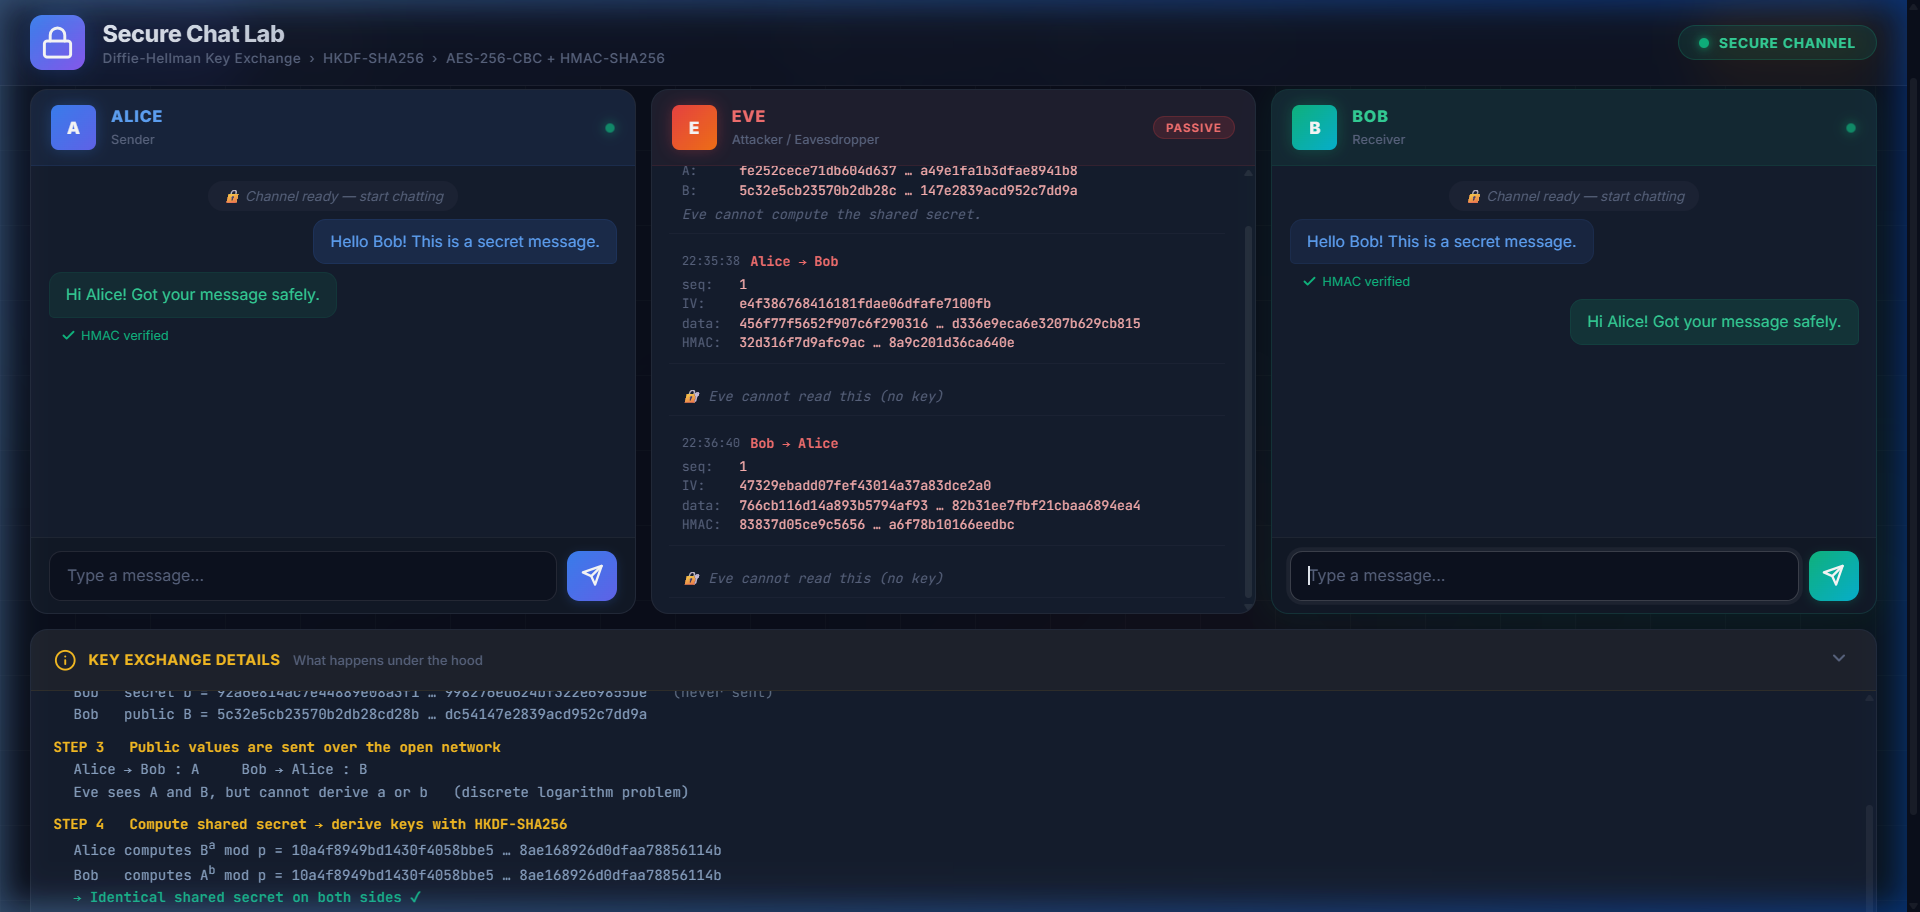
\includegraphics[width=0.88\linewidth]{screenshots/fig3_alice_bob_chat.png}
    \caption{Confidential message exchange with eavesdropper wire view.}
    \label{fig:exp_chat}
\end{figure}
\noindent \textbf{Analysis:} Plaintext messages are displayed with green HMAC verification badges on legitimate endpoints. Meanwhile, Eve captures only the sequence counter, random IV, high-entropy AES ciphertext, and HMAC tag. Eve's log indicates: \textit{"Eve cannot read this (no key)"}.

\newpage
\subsection{Figure 4: Active Ciphertext Tampering Attack (Rejected by HMAC)}
\begin{figure}[H]
    \centering
    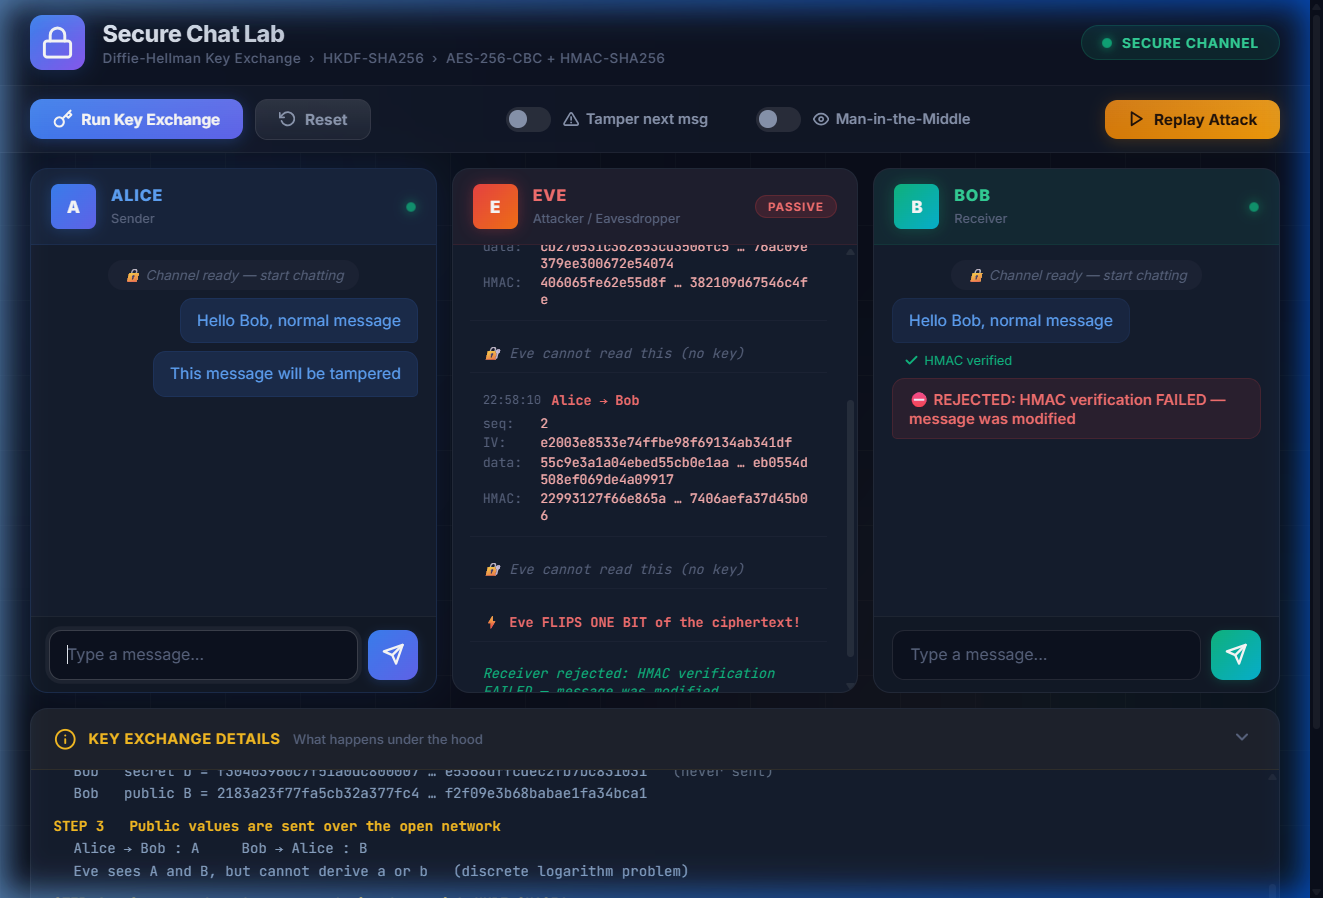
\includegraphics[width=0.88\linewidth]{screenshots/fig4_tamper_attack_rejected.png}
    \caption{Single-bit tampering detected and rejected by HMAC verification.}
    \label{fig:exp_tamper}
\end{figure}
\noindent \textbf{Analysis:} Eve flips bit 0 of byte 26 in transit. Bob recomputes HMAC-SHA256 over the wire payload; verification fails immediately. Bob displays \texttt{REJECTED: HMAC verification FAILED - message was modified}, completely preventing corrupted payload decryption.

\subsection{Figure 5: Replay Attack (Rejected by Anti-Replay Counter)}
\begin{figure}[H]
    \centering
    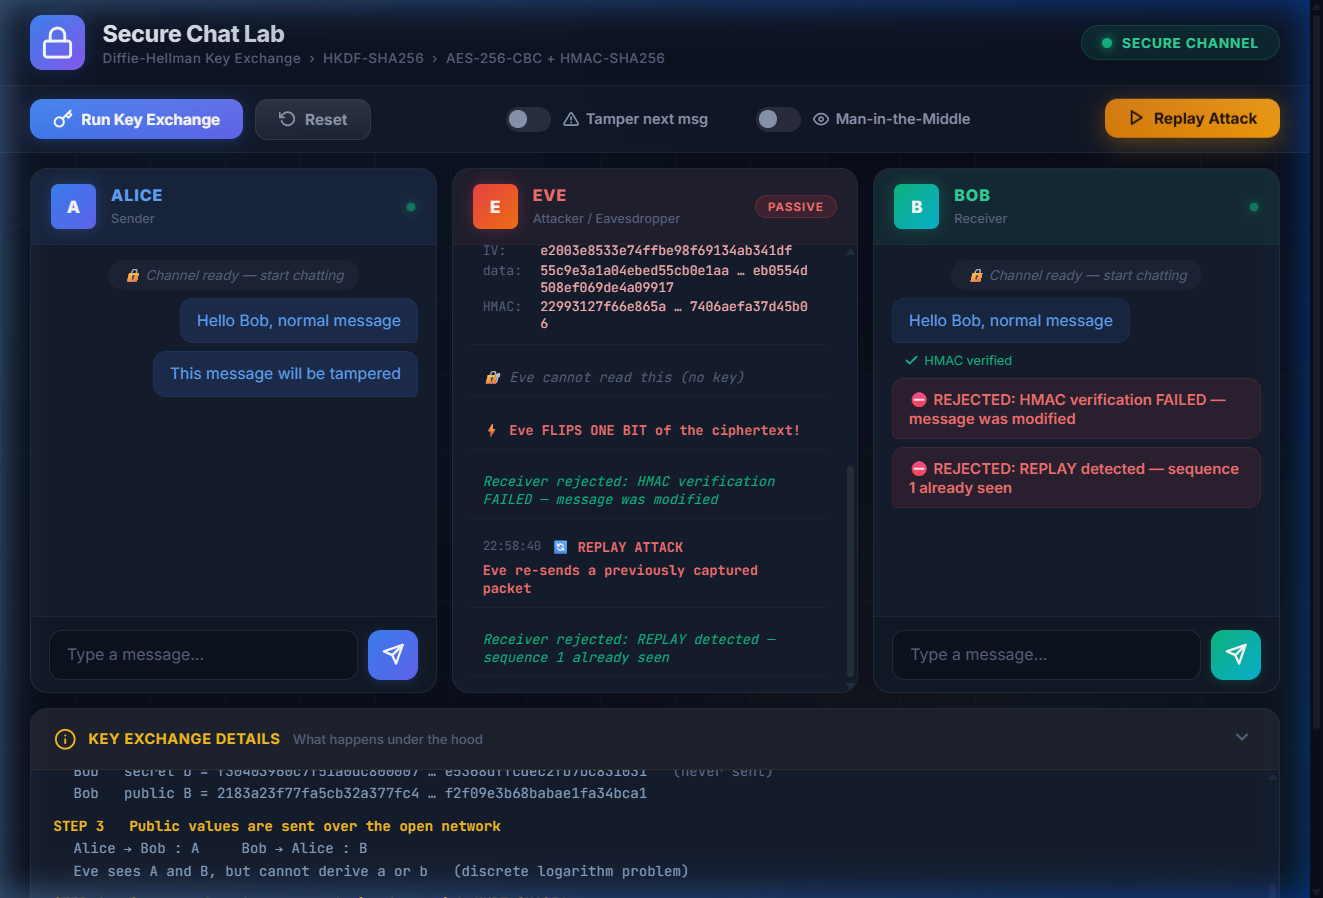
\includegraphics[width=0.88\linewidth]{screenshots/fig5_replay_attack_rejected.png}
    \caption{Replay attack blocked by monotonic sequence counter verification.}
    \label{fig:exp_replay}
\end{figure}
\noindent \textbf{Analysis:} Eve re-injects a previously valid packet into the wire. Bob's HMAC verification passes, but the freshness check determines that $\text{Seq} \le \text{Recv\_Seq}$. The packet is dropped with: \texttt{REJECTED: REPLAY detected - sequence 1 already seen}.

\newpage
\subsection{Figure 6: Unauthenticated DH Man-in-the-Middle (MITM) Interception}
\begin{figure}[H]
    \centering
    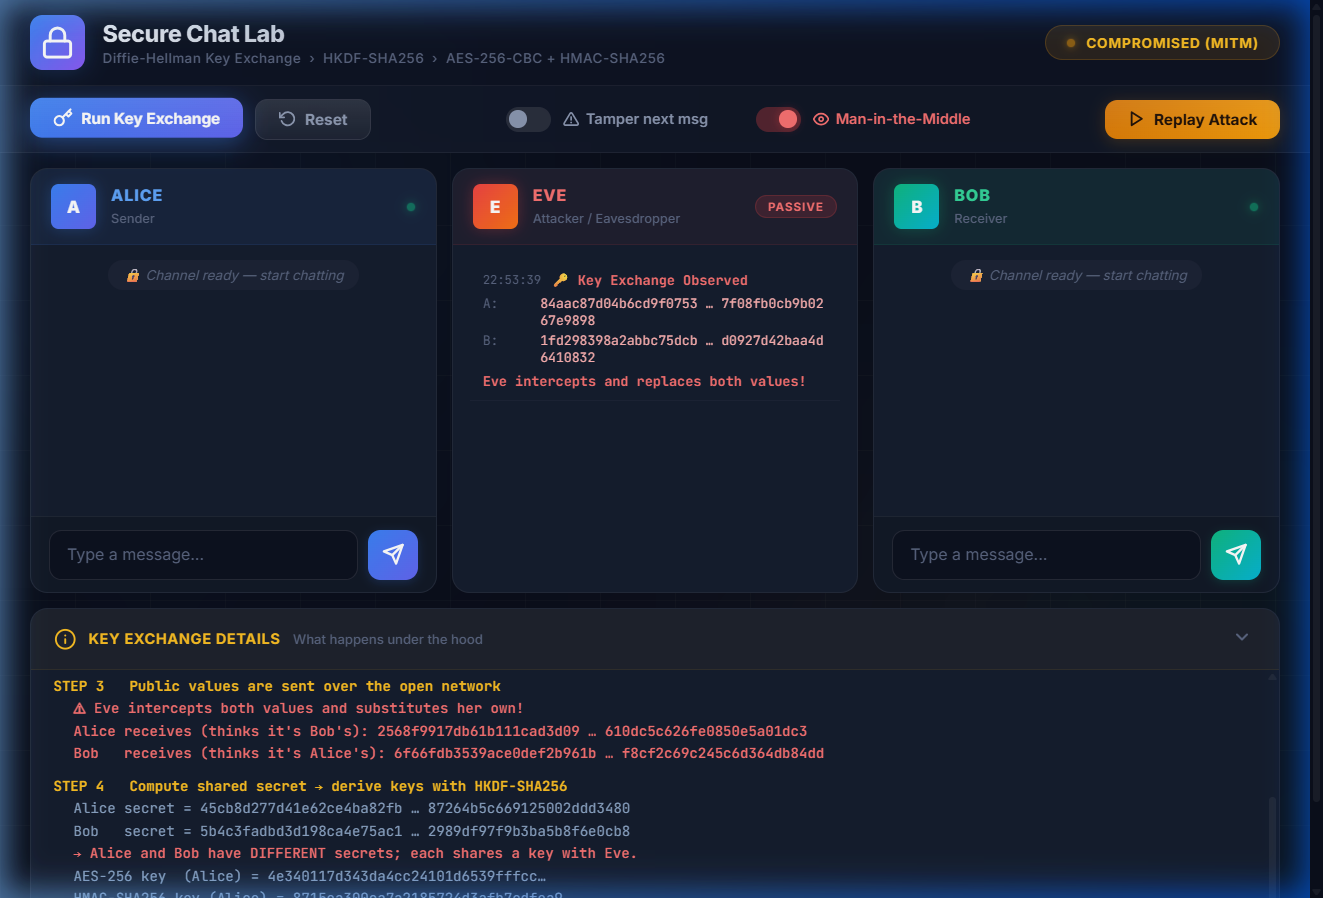
\includegraphics[width=0.88\linewidth]{screenshots/fig6_mitm_exchange.png}
    \caption{Eve intercepts and substitutes public keys during DH handshake.}
    \label{fig:exp_mitm_kx}
\end{figure}
\noindent \textbf{Analysis:} With MITM active, Eve intercepts Alice's public key $A$ and Bob's public key $B$, substituting her own generated keys $Y_{E_1}$ and $Y_{E_2}$. Alice and Bob establish separate keys with Eve while believing they are directly paired. The badge signals \texttt{COMPROMISED (MITM)}.

\subsection{Figure 7: MITM Traffic Eavesdropping and Payload Manipulation}
\begin{figure}[H]
    \centering
    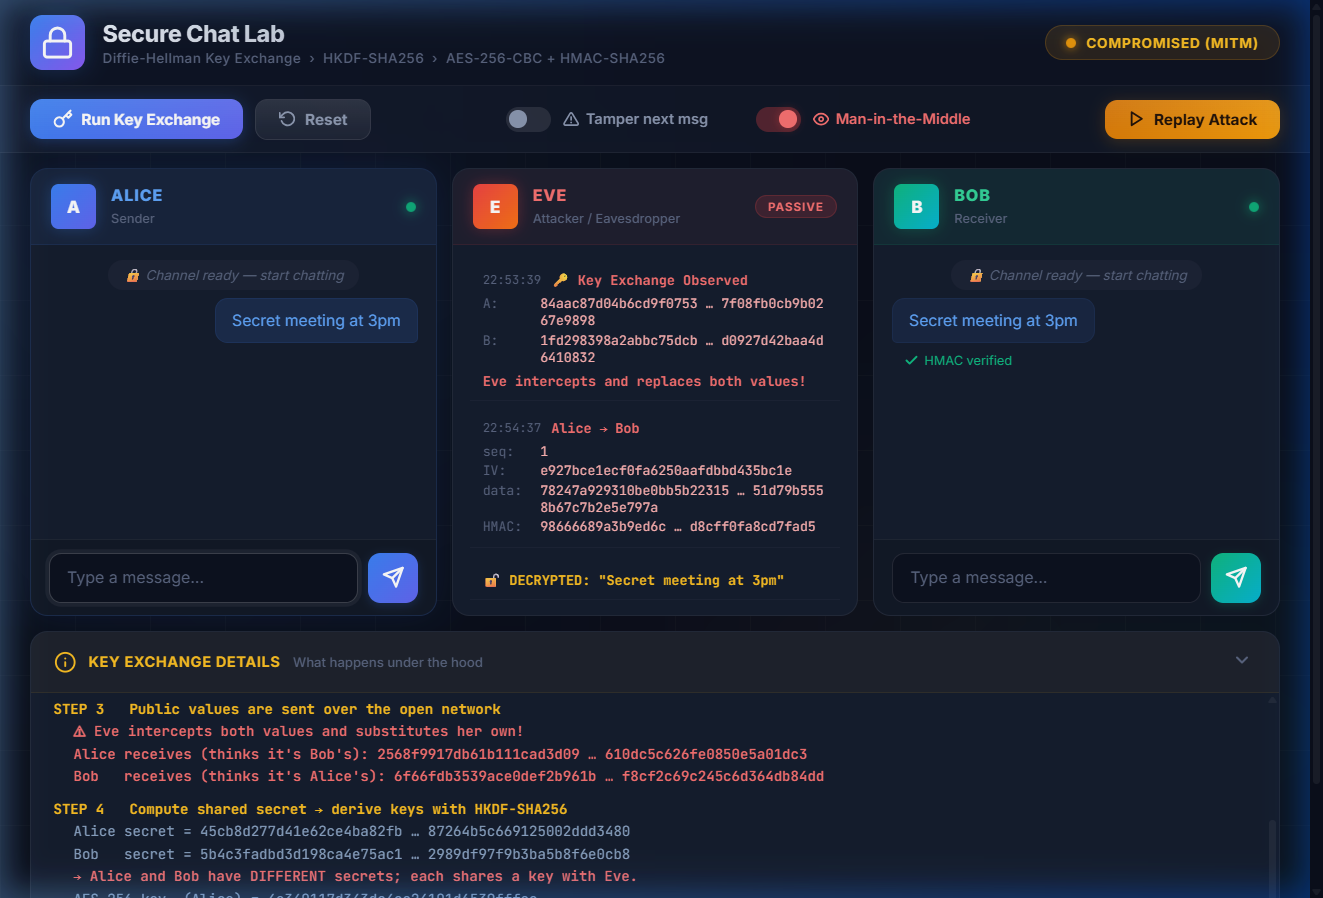
\includegraphics[width=0.88\linewidth]{screenshots/fig7_mitm_intercepted_message.png}
    \caption{Eve decrypts, modifies, and re-encrypts ciphertext in transit.}
    \label{fig:exp_mitm_msg}
\end{figure}
\noindent \textbf{Analysis:} Alice sends \texttt{"Secret meeting at 3pm"}. Eve decrypts the payload using $K_{AE}$, reads the plaintext in clear, appends \texttt{[edited by Eve]}, re-encrypts using $K_{EB}$, and forwards it to Bob. Bob receives the modified text with a valid tag, proving that \textbf{unauthenticated Diffie-Hellman does not provide peer authentication}.

% ==============================================================================
% SECTION 6: IMPLEMENTATION CODE
% ==============================================================================
\section{Implementation Code}

The project implementation encompasses the complete cryptographic core, packet assembly, and tri-party interactive GUI. Below is the source code of \texttt{secure\_chat\_lab.py}:

\begin{lstlisting}[language=Python, caption={Python Cryptographic Engine and Protocol Pipeline (secure\_chat\_lab.py)}]
import os
import struct
import time
import tkinter as tk
from tkinter import ttk

from cryptography.hazmat.primitives import hashes, hmac, padding
from cryptography.hazmat.primitives.asymmetric import dh
from cryptography.hazmat.primitives.ciphers import Cipher, algorithms, modes
from cryptography.hazmat.primitives.kdf.hkdf import HKDF
from cryptography.exceptions import InvalidSignature

# RFC 3526 group 14 (2048-bit MODP safe prime), generator g = 2
P_HEX = (
    "FFFFFFFFFFFFFFFFC90FDAA22168C234C4C6628B80DC1CD129024E088A67CC74"
    "020BBEA63B139B22514A08798E3404DDEF9519B3CD3A431B302B0A6DF25F1437"
    "4FE1356D6D51C245E485B576625E7EC6F44C42E9A637ED6B0BFF5CB6F406B7ED"
    "EE386BFB5A899FA5AE9F24117C4B1FE649286651ECE45B3DC2007CB8A163BF05"
    "98DA48361C55D39A69163FA8FD24CF5F83655D23DCA3AD961C62F356208552BB"
    "9ED529077096966D670C354E4ABC9804F1746C08CA18217C32905E462E36CE3B"
    "E39E772C180E86039B2783A2EC07A28FB5C55DF06F4C52C9DE2BCBF695581718"
    "3995497CEA956AE515D2261898FA051015728E5A8AACAA68FFFFFFFFFFFFFFFF"
)
P = int(P_HEX, 16)
G = 2
PARAMS = dh.DHParameterNumbers(P, G).parameters()

class Keys:
    """AES key + HMAC key derived from one shared secret via HKDF."""
    def __init__(self, shared_secret: bytes):
        okm = HKDF(hashes.SHA256(), 64, salt=None,
                   info=b"secure-chat-lab").derive(shared_secret)
        self.aes_key, self.mac_key = okm[:32], okm[32:]
        self.send_seq = 0
        self.recv_seq = 0

def encrypt_message(keys: Keys, text: str) -> bytes:
    """packet = seq(8) | iv(16) | ciphertext | hmac(32)"""
    keys.send_seq += 1
    seq = struct.pack(">Q", keys.send_seq)
    iv = os.urandom(16)
    padder = padding.PKCS7(128).padder()
    padded = padder.update(text.encode()) + padder.finalize()
    enc = Cipher(algorithms.AES(keys.aes_key), modes.CBC(iv)).encryptor()
    ct = enc.update(padded) + enc.finalize()
    h = hmac.HMAC(keys.mac_key, hashes.SHA256())
    h.update(seq + iv + ct)
    return seq + iv + ct + h.finalize()

def decrypt_message(keys: Keys, packet: bytes, check_replay=True) -> str:
    """Verify HMAC first, then replay check, then decrypt."""
    if len(packet) < 8 + 16 + 16 + 32:
        raise ValueError("packet too short")
    seq, iv, ct, tag = packet[:8], packet[8:24], packet[24:-32], packet[-32:]
    h = hmac.HMAC(keys.mac_key, hashes.SHA256())
    h.update(seq + iv + ct)
    try:
        h.verify(tag)
    except InvalidSignature:
        raise ValueError("HMAC verification FAILED - message was modified")
    n = struct.unpack(">Q", seq)[0]
    if check_replay and n <= keys.recv_seq:
        raise ValueError(f"REPLAY detected - sequence {n} already seen")
    dec = Cipher(algorithms.AES(keys.aes_key), modes.CBC(iv)).decryptor()
    padded = dec.update(ct) + dec.finalize()
    unpadder = padding.PKCS7(128).unpadder()
    text = unpadder.update(padded) + unpadder.finalize()
    if check_replay:
        keys.recv_seq = n
    return text.decode()

class Party:
    """One communication participant (Alice, Bob, or Eve's fake persona)."""
    def __init__(self, name):
        self.name = name
        self.priv = PARAMS.generate_private_key()
        self.x = self.priv.private_numbers().x
        self.y = self.priv.public_key().public_numbers().y
        self.keys = None

    def compute_shared(self, peer_y: int) -> bytes:
        peer = dh.DHPublicNumbers(peer_y, PARAMS.parameter_numbers()).public_key()
        secret = self.priv.exchange(peer)
        self.keys = Keys(secret)
        return secret
\end{lstlisting}

% ==============================================================================
% SECTION 7: SECURITY DISCUSSION
% ==============================================================================
\section{Security Discussion \& Theoretical Guarantees}

\subsection{Why Encrypt-then-MAC (EtM)?}
Classical protocols historically experimented with three generic composition paradigms:
\begin{itemize}[leftmargin=1cm]
    \item \textbf{MAC-then-Encrypt (MtE):} (Used in TLS 1.0--1.2). $C = E(P \parallel \text{MAC}(P))$. Vulnerable to timing side-channels and padding oracle attacks (e.g., Lucky Thirteen).
    \item \textbf{Encrypt-and-MAC (E\&M):} (Used in SSH). $C = E(P), T = \text{MAC}(P)$. The MAC tag can leak information about the plaintext because MACs are not guaranteed to be pseudorandom.
    \item \textbf{Encrypt-then-MAC (EtM):} (Used in IPsec, TLS 1.3, Signal). $C = E(P), T = \text{MAC}(C)$. Proven by Krawczyk (2001) to achieve IND-CCA2 security generically under any secure symmetric cipher and PRF MAC.
\end{itemize}

\subsection{Mitigating Diffie-Hellman MITM Attacks}
The project's MITM simulation demonstrates that while Diffie-Hellman provides computational secrecy against passive eavesdroppers, \textbf{it does not provide peer entity authentication}. To prevent MITM in production environments:
\begin{enumerate}[leftmargin=1cm]
    \item \textbf{Digital Signatures (PKI):} Ephemeral DH public keys ($A, B$) are signed using long-term asymmetric keys (e.g., ECDSA or Ed25519) certified by an X.509 Certificate Authority, exactly as in TLS 1.3.
    \item \textbf{Out-of-Band Safety Numbers:} Modern secure messaging protocols (e.g., Signal, WhatsApp) compute a cryptographic fingerprint over both public keys:
    \begin{equation}
        \text{Fingerprint} = \text{SHA-512}(A \parallel B)
    \end{equation}
    Users verify this hash through QR codes or verbal confirmation.
\end{enumerate}

% ==============================================================================
% SECTION 8: CONCLUSION
% ==============================================================================
\section{Conclusion}
This project successfully designed, analyzed, and implemented a robust, end-to-end secure communication system embodying modern cryptographic standards. By pairing RFC 3526 2048-bit Diffie-Hellman key exchange with HKDF-SHA256, AES-256-CBC, and Encrypt-then-MAC HMAC-SHA256 with sequence freshness verification, the architecture achieves confidentiality, data integrity, origin authenticity, and anti-replay protection. The tri-party visual attack simulation clearly demonstrates the operational mechanics of real-world cryptographic defense against passive eavesdropping, active payload tampering, replay attacks, and man-in-the-middle vulnerabilities.

% ==============================================================================
% REFERENCES
% ==============================================================================
\section*{References}
\addcontentsline{toc}{section}{References}

\begin{enumerate}[leftmargin=1cm, label={[\arabic*]}]
    \item Diffie, W., \& Hellman, M. (1976). New directions in cryptography. \textit{IEEE Transactions on Information Theory}, 22(6), 644--654.
    \item Kivinen, T., \& Kojo, M. (2003). \textit{More Modular Exponential (MODP) Diffie-Hellman groups for Internet Key Exchange (IKE)}. RFC 3526, Internet Engineering Task Force (IETF).
    \item Krawczyk, H., \& Eronen, P. (2010). \textit{HMAC-based Extract-and-Expand Key Derivation Function (HKDF)}. RFC 5869, Internet Engineering Task Force (IETF).
    \item Krawczyk, H. (2001). The order of encryption and authentication for protecting communications (or: How secure is SSL?). In \textit{Advances in Cryptology --- CRYPTO 2001} (pp. 310--331). Springer, Berlin, Heidelberg.
    \item Bellare, M., \& Namprempre, C. (2000). Authenticated encryption: Relations among notions and analysis of the generic composition paradigm. In \textit{Advances in Cryptology --- ASIACRYPT 2000} (pp. 531--545). Springer, Berlin, Heidelberg.
    \item National Institute of Standards and Technology (NIST). (2001). \textit{Advanced Encryption Standard (AES)}. Federal Information Processing Standards Publication (FIPS PUB 197).
    \item National Institute of Standards and Technology (NIST). (2001). \textit{Recommendation for Block Cipher Modes of Operation: Methods and Techniques}. NIST Special Publication 800-38A.
    \item Krawczyk, H., Bellare, M., \& Canetti, R. (1997). \textit{HMAC: Keyed-Hashing for Message Authentication}. RFC 2104, Internet Engineering Task Force (IETF).
    \item Stallings, W. (2017). \textit{Cryptography and Network Security: Principles and Practice} (7th ed.). Pearson Education.
    \item Rescorla, E. (2018). \textit{The Transport Layer Security (TLS) Protocol Version 1.3}. RFC 8446, Internet Engineering Task Force (IETF).
\end{enumerate}

\end{document}
